\documentclass[12pt]{article}
%General Packages
\usepackage{multicol, enumerate, enumitem, hyperref, color, soul, setspace, parskip, fancyhdr}

%Math Packages
\usepackage{amssymb, amsthm, amsmath, bbm, latexsym, units, mathtools}

%All math in Display Style
\everymath{\displaystyle}

% Packages with additional options
\usepackage[headsep=0.5cm,headheight=0cm, left=1 in,right= 1 in,top= 1 in,bottom= 1 in]{geometry}
\usepackage[usenames,dvipsnames]{xcolor}

% SageTeX
\usepackage{sagetex}

% Package to use the command below to create lines between items
\usepackage{dashrule}
\newcommand{\litem}[1]{\item#1\hspace*{-1cm}\rule{\textwidth}{0.4pt}}

\pagestyle{fancy}
	\lhead{Module 4 - Quadratic Equations}
	\chead{}
	\rhead{Progress Exam 3}
	\lfoot{Spring 2019}
	\cfoot{}
	\rfoot{Version B}

\begin{document}
	\pagestyle{fancy}

\begin{sagesilent} 
load("../Code/generalPurposeMethods.sage")
load("../Code/keyGeneration.sage")
\end{sagesilent}

\begin{enumerate}
\setcounter{enumi}{15}
%OBJECTIVE 1 - Convert between a quadratic function and its graph.
\begin{sagesilent}
moduleNumber = 4
version = "B"
problemNumber = 16
load("../Code/quadratic/quadraticGraphs.sage")
\end{sagesilent}
% TYPE 1 - Graph to function

\litem{ \sage{displayStem1}

	\begin{center}
	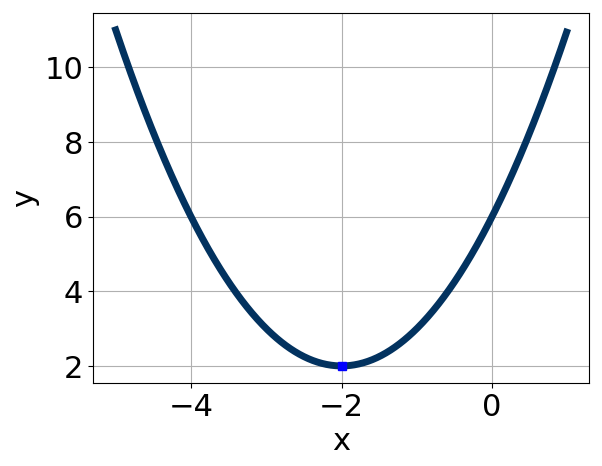
\includegraphics[width = 0.35\textwidth]{../Figures/question16B.png}
	\end{center}
	\vspace*{-3mm}
	\hspace*{10mm} $a =$ \framebox(30,20){} \hspace*{10mm} $b =$ \framebox(30,20){} \hspace*{10mm} $c =$ \framebox(30,20){}
	\begin{enumerate}[label=\Alph*.]
		\item $\sage{choices[0]}$
		\item $\sage{choices[1]}$
		\item $\sage{choices[2]}$
		\item $\sage{choices[3]}$
		\item $\sage{choices[4]}$
	\end{enumerate}	\vspace*{-5mm}
}

% TYPE 2 - Function to graph
\litem{ Graph the equation $f(x)= \sage{functionToGraph}. $
\begin{multicols}{2}
	\begin{enumerate}[label=\Alph*.]
		\item 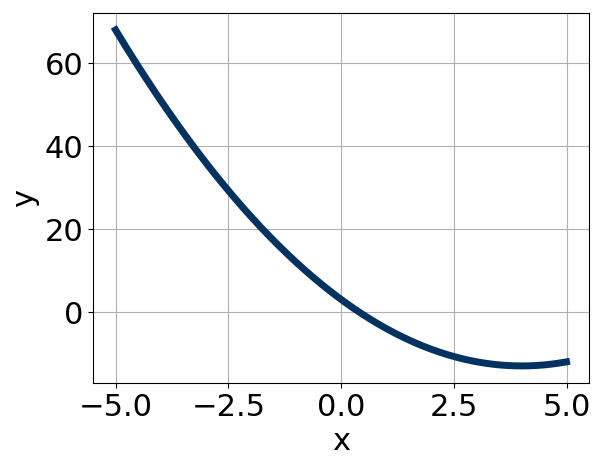
\includegraphics[width = 0.25\textwidth]{../Figures/question17AB.png}
		\item 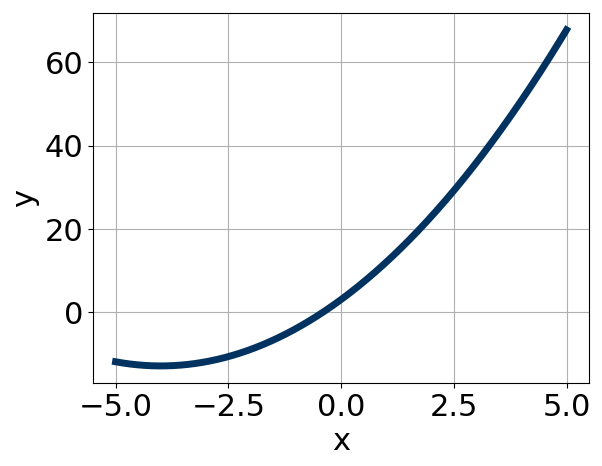
\includegraphics[width = 0.25\textwidth]{../Figures/question17BB.png}
		\item 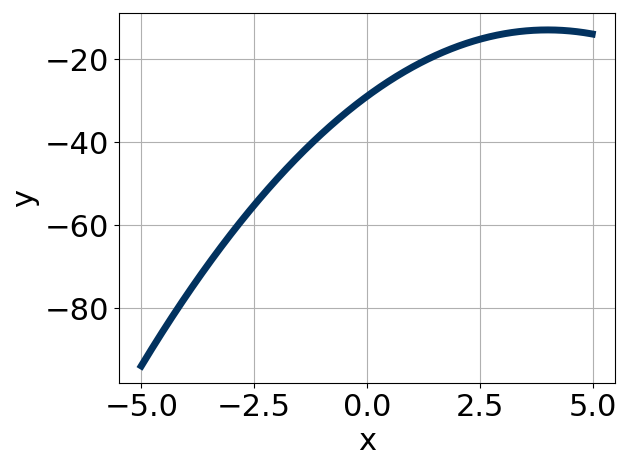
\includegraphics[width = 0.25\textwidth]{../Figures/question17CB.png}
		\item 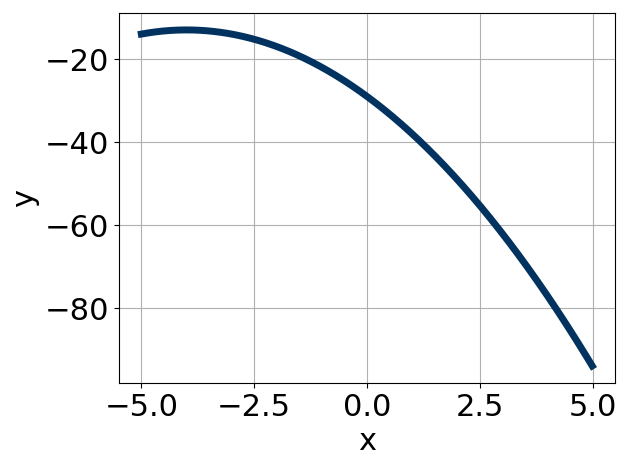
\includegraphics[width = 0.25\textwidth]{../Figures/question17DB.png}
		\item 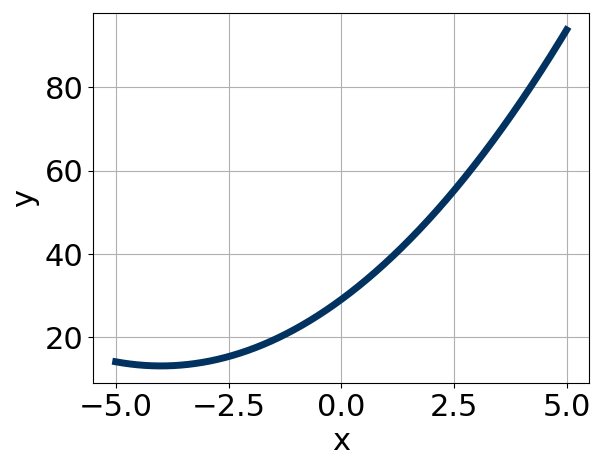
\includegraphics[width = 0.25\textwidth]{../Figures/question17EB.png}
	\end{enumerate}	\vspace*{-5mm}
\end{multicols}
}

\begin{sagesilent}
problemNumber = 18
load("../Code/quadratic/factorLeadingOver1Composite.sage")
\end{sagesilent}
%Factor - a and c are fairly composite (ac has at least 8 factors)
\litem{ \sage{displayStem}	

	$$\sage{displayProblem}$$
\hspace*{5mm} $a =$ \framebox(30,20){} \hspace*{5mm} $b =$ \framebox(30,20){} \hspace*{5mm} $c =$ \framebox(30,20){} \hspace*{5mm} $d =$ \framebox(30,20){}
	\begin{enumerate}[label=\Alph*.]
		\item $\sage{choices[0]}$
		\item $\sage{choices[1]}$
		\item $\sage{choices[2]}$
		\item $\sage{choices[3]}$
		\item $\sage{choices[4]}$
	\end{enumerate}	
						
}

\begin{sagesilent}
problemNumber = 19
load("../Code/quadratic/solveQuadraticFactorComposites.sage")
\end{sagesilent}
%TYPE 2 (Type 3 from M2O4) - a and c are fairly composite (ac has at least 8 factors)
\litem{ \sage{displayStem} \vspace*{-3mm}
	$$ \sage{generalFormTypeTwo} = 0$$
\hspace*{10mm} $x_1 =$ \framebox(30,20){} \hspace*{20mm} $x_2 =$ \framebox(30,20){}
	\begin{enumerate}[label=\Alph*.]
		\item $\sage{choices[0]}$
		\item $\sage{choices[1]}$
		\item $\sage{choices[2]}$
		\item $\sage{choices[3]}$
		\item $\sage{choices[4]}$
	\end{enumerate}	\vspace*{-3mm}

}


%OBJECTIVE 3 - Solve quadratic equations using the Quadratic Formula
\begin{sagesilent}
problemNumber = 20
load("../Code/quadratic/quadraticFormula.sage")
\end{sagesilent}
% FOR NOW, let's avoid complex roots and just let students reduce irrational solutions to decimal form. They are allowed calculators, so this will be fine.
\litem{ \sage{displayStem}
	$$ \sage{problemQuadraticFormula} = 0 $$
\hspace*{10mm} $x_1 =$ \framebox(30,20){} \hspace*{20mm} $x_2 =$ \framebox(30,20){}
	\begin{enumerate}[label=\Alph*.]
		\item $\sage{choices[0]}$
		\item $\sage{choices[1]}$
		\item $\sage{choices[2]}$
		\item $\sage{choices[3]}$
		\item $\sage{choices[4]}$
	\end{enumerate}	
}

\end{enumerate}

\end{document}